%!TEX root = ../../main.tex

\chapter{Introduction}
These days one of the key benchmarks for technology is processing speed and
calculation power. To realize mathematical operations and execute programs,
different platforms can be utilized. The most commonly used unit is the standard
processor consisting of transistors realized on silicium and other materials.
Another crucial technology that is gaining more attention is the so-called
\acf{FPGA}. The FPGA consists of logical units that can
be wired and configured individually for the required use-case. The advantage of
FPGA is that the speed of applications can be drastically increased since the
hardware will be very optimized for the specific application.
This project aims to develop a \acf{IP}-core based on the Open
Source Instruction Set \acs{RISC}-V. The goal is to build a reusable unit of logic that can
interpret compiled C-Code. The IP core is realized in the \ac{VHDL} language and will be deployed on a FPGA. IP Cores are used in every computer, phone and electronic device that requires to execute some computational function. The developers of these IP Cores are big
companies like Intel, ARM or AMD. These IP Cores and Instruction Sets are strictly
licensed and not available for everyone. For the development of an own IP Core the
Instruction Set is the main source of information and therefore the RISC-V
open-source Instruction Set is used for this project.
\section{Motivation}
RISC-V was first proposed at Berkeley University in 2010. The architecture is
therefore relatively new in comparison to others like x86, ARM or SPARC. Even
though its young age is already very promising, every year new breakthroughs are
achieved in the field of RISC-V based cores.
MicroMagic for example announced in 2020 a chip with a total CoreMark score of
13000 and an incredible 110000 Coremark/Watt. This poses a significant
development and is approximately 10 times better than any CISC, RISC or MIPS
implementation in terms of Performance per Watt.
Many other companies like Alibaba, Nvidia and SiFive are currently increasing
research on RISC-V based cores.
The Motivation behind this project was to gain experience in processor and \ac{FPGA}
design and verification. Furthermore it poses an interesting opportunity for students
to work on a new and upcoming processor architecture.

\section{Project Planning}
In order to control the flow of the project, the V-Model approach was taken. The
project is therefore divided into Requirements, System Design, Architecture Design,
Module Design and Implementation. After Implementation the corresponding
verification phases are ready to be executed, starting from the lowest level (Unit
Verification) to Integration Verification, System Verification and last but not least
Acceptance Verification.


\begin{figure}[h]
	\centering
	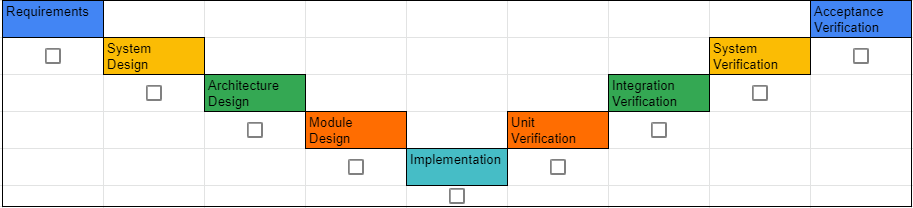
\includegraphics[scale=0.65]{vmod.png}
	\caption{V-Model}
\end{figure}

At the beginning of every project phase, workloads were defined e.g. the definition of
the Control Unit Entity. The target of Requirements Engineering was to define
everything that is expected from the core and gather information about RISC-V. The
data path as well as the entities of the Control Unit, Arithmetic Unit, Register Files,
Exception Control, \acs{PMP} \& \acs{PMA} Checker and AXI4-Lite Interfaces as well as a short
summary of their function were defined during System Design. The next step,
Architecture Design, aimed to further specify the entities mentioned above and
sub-divide them into several entities. Module Design will be executed to define every
single architecture, after that implementation and testing may start.

\section{History}

